\documentclass[../main.tex]{subfiles}

\begin{document}
\section{Detecting spectral pollution}

\subsection{Dissipative barrier methods}\label{sec:dissipative-barrier}
Perhaps one of the simplest methods for separating eigenvalues from spectral pollution is the dissipative barrier method.
This method leverages finite-rank perturbation of an operator.

Take an operator $T$ on a Hilbert space, and
let $P$ be an orthonormal projection onto a finite-dimensional space  such that for an eigenvector $u$, $\|Pu - u\|$ is sufficiently small.
Let $\lambda$ be the eigenvalue for $u$. Then for the operator $T+iP$,

$$(T+iP) u = Tu + iPu \approx \lambda u + iu = (\lambda + i)u.$$

i.e. $(\lambda + i)$ is approximately an eigenvalue for $T+iP$. 

Then, the eigenvalues of the perturbed operator will have imaginary part of approximately 1, and the set of eigenvalues produced by the approximation 
can be filtered to discard points without imaginary part close to 1 as being pollution. This is particularly useful for self-adjoint operators, where the entire spectrum and the essential numerical range are a subset of the real line; in that case, the perturbed eigenvalues will be the only points on the spectrum with significant imaginary part. Even better, if the operator is also bounded, then all pollution is in the essential numerical range (Theorem \ref{}) which is
invariant under compact perturbation (Theorem \ref{}) so the pollution will converge to the real axis.

Let us see this concretely with an example.

\begin{example}
We return once again to our discontinuous multiplication operator $M_f$ on $L^2(0, 1)$ with symbol
$$
f: x \mapsto \begin{cases}
x & x < 1/2\\
x+1/2 & \text{otherwise}.
\end{cases}
$$
This time, we add a `rank-one perturbation' to get the operator $\tilde{M}$ which has the action
$$\tilde{M}u = M_fu + (u, \varphi) \varphi,$$
where $\varphi$ is a real-valued function on $L^2(0, 1)$. Then $\tilde{M}$ has an eigenvector: we rearrange to get
\begin{align*}
f(x)u(x) + (u, \varphi)\varphi(x) & = \lambda u(x),\\
\text{therefore }(\lambda - f(x))u(x) & = (u, \varphi)\varphi(x),\\
u(x) & = c \frac{\varphi(x)}{\lambda - f(x)}
\end{align*}
for some constant $c$. We then normalise this to $\frac{\varphi(x)}{\lambda - f(x)}$, which requires
\begin{align*}
f(x)u + (u, \varphi)\varphi & = \lambda u \\
(f(x) - \lambda)c\frac{\varphi(x)}{\lambda - f(x)} + (\frac{c\varphi}{\lambda - f}, \varphi)\varphi(x) & = 0 \\
-1 + (\frac{\varphi}{\lambda - f}, \varphi) & = 0
\end{align*}
so we can normalise provided that $(\frac{\varphi}{\lambda - f}, \varphi) = \int_0^1 \frac{|\varphi|^2}{\lambda - m} = 1.$
\end{example}

Thus for any value $\lambda$ we can choose $\varphi \in L^2(0, 1)$ and scale it so that $\int_0^1 \frac{|\varphi|^2}{\lambda - m} = 1$
to get an operator $\tilde{M}$ with spectrum $\Spec(M) \cup \{\lambda \in \mathbb{C} : \int_0^1 \frac{|\varphi|^2}{\lambda - m} = 1\}$. In Figure \ref{fig:nodbm} we can see the results of Ritz approximations
with $\varphi$ chosen such that the operator has an eigenvalue at 0.7.\footnote{In particular, $\varphi$ was chosen to be the constant
$(\log(3) - 3\log(2) + \log(5) + \log(7) - \log(10))^{-1}$; this satisfies the normalisation condition at $\lambda = 0.7$ but also at $\lambda \approx 4.4$;
the eigenvalue at $\lambda \approx 4.4$ has been cropped out of the figure to improve illustration of the idea.} In Figure \ref{fig:dbm} we see the same approximation but with the dissipative barrier $iP$ where $P$ is the projection onto $\mathrm{span}\{\phi_n, |n| \leq 25\}$. Note that the spectrum on the line ${(x, y) : \mathrm{Imag}(x) = 1}$ converges to what we'd expect the spectrum to be!

\begin{figure}[p!]
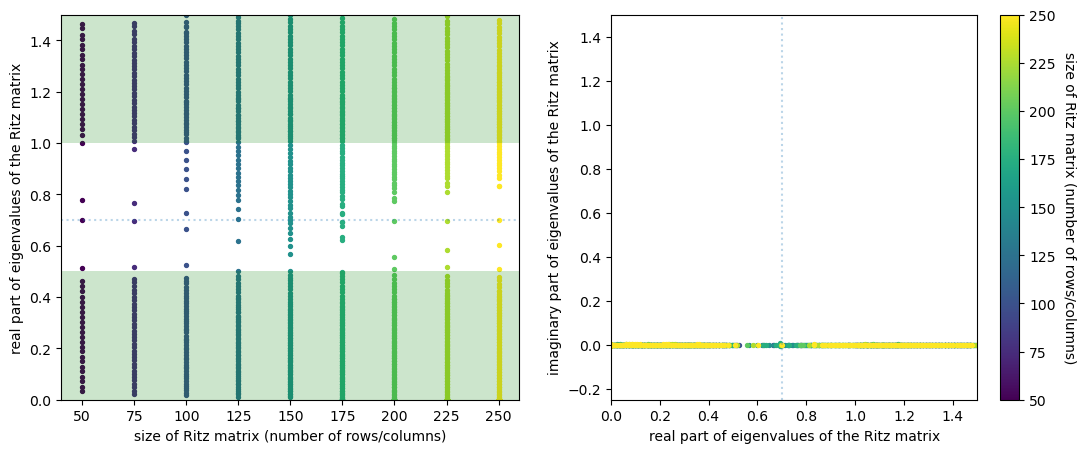
\includegraphics[width=0.9\linewidth, height=6cm]{ptb-mult-nodbm}
\caption{The real part of the approximate spectrum for $\tilde{M}$; on the left, the real parts of the approximate spectrum as the size of the Ritz matrix increases;
on the left, the complex approximate spectrum where colour is used to donate the size of the approximation. The green shaded regions correspond to
the essential spectrum of $\tilde{M}$, and the dotted lines are at $\mathrm{Re}(x) = 0.7$ to show where the added eigenvalue should be. 
(An intuitive way to view these figures is to see them as a three-dimensional plot, with the left figure `top-down', and the right figure `from the east')}
\label{fig:nodbm}
\end{figure}

\begin{figure}[p!]
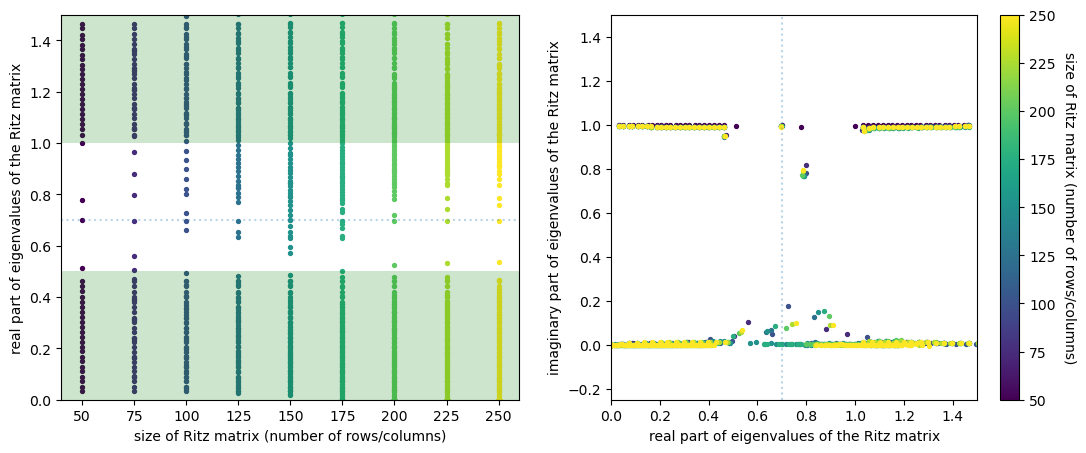
\includegraphics[width=0.9\linewidth, height=6cm]{ptb-mult-dbm} 
\caption{The real part of the approximate spectrum for $\tilde{M}+iP$; compare with Figure \ref{fig:nodbm}. See that the line at 1.0 on the imaginary
axis converges to the actual spectrum of the operator, while the pollution remains below.}
\label{fig:dbm}
\end{figure}
\clearpage

\begin{remark}
One may also note that there are bands corresponding to the essential spectrum with imaginary part 1. 
The reason why dissipative barriers `replicate' the essential spectrum is an open problem; it has recently been investigated specifically for Schr\"odinger operators \cite{stepanenkoTODO} but in general remains unknown.
\end{remark}

As a second example, let us try to replicate some results from Aceto et al. (2006) \cite{aceto2006numerical}. In this paper, they use an algebraic method
combined with a `shooting technique' to find high-accuracy estimates of eigenvalues for a Sturm-Liouville operator; this highly-specialised algorithm
is free from pollution but works only for a specific class of Sturm-Liouville operators.
is a 

\begin{example}\label{ex:aceto}
In particular, take the following eigenvalue problem on $L^2[0, \infty)$:

$$
\begin{cases}
-y'' + (\sin(x) - \frac{40}{1+x^2})y = \lambda y \\
y(0) \cos(\pi/8) + y'(0) \cos(\pi/8) = 0.
\end{cases}
$$

This operator has a `band-gap' structure; it has intervals (bands) of essential spectrum, with eigenvalues dotted in the gaps between bands.
In two of the spectral gaps $J_2 = (-0.34767, 0.59480)$ and $J_3 = (0.91806, 1.2932)$ (denoted in line with the paper and rounded to 5sf) the
algebraic method finds the following eigenvalues:

\begin{figure*}[h!]
\centering
\begin{tabular}{c c}
$J_2$ & $J_3$ \\
\hline\hline
0.33594 & 0.94963 \\
0.53662 & 1.2447 \\
0.58083 & 1.2919 \\
0.59150 & \\
\end{tabular}
\end{figure*}

Firstly, we will see whether we can reproduce this data. The algebraic method used first truncates the half-line to $[0, 70\pi]$. We will do the same and
perform a Ritz approximation on the truncated interval, applying a dissipative barrier; this is a success, as one can see in Figure \ref{fig:aceto-dbm}.

Now we will aim for better; whether we can reproduce these eigenvalues using a Ritz approximation on $[0, \infty)$, with the orthonormal basis $\{\phi_n\}_{n \in \mathbb{N}},
\phi_n = \exp(-x/2)L_n$, where $L_n$ is the n'th Laguerre polynomial (see \cite{szego1975orthogonal} for a proof that this is indeed an orthonormal basis)
\end{example}

\begin{figure}[p!]
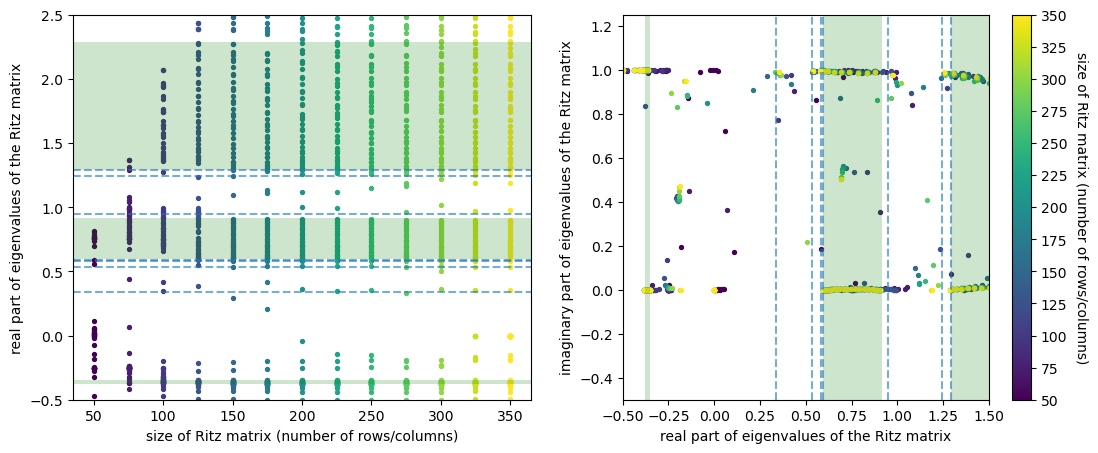
\includegraphics[width=0.9\linewidth, height=6cm]{aceto-dbm}
\caption{The results of truncating the domain and applying a dissipative barrier to the operator of Example \ref{ex:aceto}.
The green bands represent the essential spectrum of the operator, and the dotted blue lines indicate where the algebraic method found
eigenvalues in two spectral gaps. Note that for larger approximations, the points in the spectral gaps with imaginary part 1.0 are
very close to the algebraic method's approximation.}
\label{fig:aceto-dbm}
\end{figure}

\subsection{Eigenvector analysis}
If we want to tell whether a particular 


\end{document}